\chapter{Filtering tags}
\begin{quotation}
\noindent
The study performed in Chap. \ref{chap:topicir} demonstrated that user tags collected with \textit{Waisda?} are not well suited for retrieving video fragments based on topic. While the search recall is satisfactory the search precision leaves much to be desired. This is mainly caused by the presence of user tags which are not valid topical annotations. In this chapter we aim to characterize the quality of the user tags and in effect detect and filter out the bad ones. We explore several features of the tags which could serve as an indication of their quality as topical descriptors. Namely, the TF-IDF score of the tags, the reputation of the players that contributed them and the tag frequency just to name a few. To measure the extend to which the tag features are effective at recognizing the bad tags we use a quantitative system evaluation methodology and an evaluation dataset that was created in the study from Chap. \ref{chap:topicir}. Our findings suggest that the TF-IDF score of the tags is a good predictor of their quality. In fact, exploiting the top ranked tags w.r.t their TF-IDF score for search can emulate the retrieval performance of the best performing system that does not utilize the user tags for search. 
\end{quotation}

Previously, in Chap. \ref{chap:topicir} we investigated how well the tags collected with \textit{Waisda?} are performing with respect to topical search. The general conclusion was that when it comes to using \textit{Waisda?} tags to retrieve fragments that are about a given topic the search performance is  unsatisfactory. This conclusion came with the following caveat: while the search recall is relatively high ($\approx$ 59\%), the search precision is rather low ($\approx$ 16\%). What this means is that a significant portion of topics covered by the fragments are in fact entered as tags by the \textit{Waisda?} players hence the high recall. Moreover, there are also \textit{bad}\footnote{The \textit{good} and \textit{bad} tag quality dichotomy is defined with respect to topical relevance. A good/bad tag is one that is topically relevant/not relevant for the fragment.} tags that do not refer to the topics covered by the fragments and when these tags result in a hit the overall search precision goes down. This being said, should the bad tags be detected and filtered out from the collection, that would result in increased precision and unchanged recall. Therefore, in this chapter we address the following research question
\begin{quote}
\textit{Can bad tags be detected and filtered out, and consequently the search performance improved?}
\end{quote} 

\paragraph{Tag Filters.} To make our discussion more precise 	we introduce the notion of \textit{tag filter}. Speaking formally, a tag filter $F: \mathcal{T}\rightarrow\{true, false\}$ is a unary boolean-valued function defined over the set of all tags, $\mathcal{T}$. For example, we can express the notion of verified tag using tag filters. Indeed, a filter $F_{ver}$ which evaluates to true iff it is passed a verified tag as an argument can be defined in the following way.
\begin{equation*}
F_{ver}(t) = \left\{ 
	\begin{array}{rl}
	true &\mbox{ if $\exists t' \in \mathcal{T} (v(t) = v(t') \wedge l(t) = l(t') \wedge |\tau(t) - \tau(t')| < 10)$} \\
	false &\mbox{ otherwise}
	\end{array}
\right.
\end{equation*}
for every $t \in T$ where $v(\cdot)$ is a function that returns the video fragment the tag passed as an argument is attached to,  $\tau(\cdot)$ is a function that returns the time in seconds relative to the beginning of the video when the tag was entered, and $l(\cdot)$ is a function that returns the label of the tag\footnote{The label of the tag is the actual text entered by the user that contributed the tag.}. Given a video fragment $v \in \mathcal{V}$ and a tag filter $F: \mathcal{T}\rightarrow\{true, false\}$, the set of tags that remain after the filtering is denoted by $Filter:(\mathcal{V} \times \mathcal{T}\rightarrow\{true, false\})\rightarrow \mathcal{P}({T})$ which is defined as follows\footnote{$\mathcal{P}({T})$ denotes the power set of $\mathcal{T}$}

\begin{equation}
Filter(v, F) = \{t |~t \in tags(v), F(t) = true\}
\end{equation}
where $tags(\cdot)$ is a function that returns all tags attached to the fragment passed as an argument.
For instance, $Filter(v, F_{ver})$ denotes the set of all verified tags attached to video fragment $v$.
 
The rest of the chapter is structured as follows. In Sec. \ref{sec:filter:rel-work} we discuss related work. Section \ref{sec:filter:approach} outlines our approach. In Sec. \ref{filter:sec:res} and Sec. \ref{filter:sec:con} we present the results and conclusions, respectively.

\section{Related Work}\label{sec:filter:rel-work}
There is a substantial body of research work that looks into the refinement and quality assessment of the annotations of still images. Lee at al. a proposed tag refinement technique that aims at
differentiating noisy tag assignments from correct tag assignments \cite{Lee:2010:TRI:1890924.1891010}. Each tag is assigned a probability of being noisy based on the visual similarity of the images and tag co-occurrence statistics. Tags with probability below a certain threshold are discarded as noisy. 
Furthermore, in \cite{Truong:2012:CSK:2324796.2324808,Li:2008:LTR:1460096.1460126} neighbour voting schemes for determining the tag relevance are explored. In this approach a tag is considered more relevant to the image it is ascribed to, also known as the seed image, if the tag is also used to annotate the neighbouring images. The neighbourhood relation is defined in terms of the visual similarity among images. Lee at al. expands the approach by not only considering the visually similar images but the dissimilar images as well thus providing negative examples \cite{Lee:2012:TDE:2390876.2390880}. Kennedy at al. exploits visual similarity among images in a sense that tags ascribed to images by the creators of the image are used as seed annotations and are also attached to visually similar images \cite{Kennedy:2009:RTU:1631135.1631139}. Zhao at al. proposed a data-driven method to automatically determine the relatedness between a tag and the image's visual content taking into consideration the tag co-occurrence  and the visual similarity among images \cite{Zhao:2010:TRV:2174490.2174571}.
Probabilistic methods that exploit random walk based techniques have also been explored \cite{Wang:2006:IAR:1180639.1180774,Liu:2009:TR:1526709.1526757,Li:2012:TRP:2382336.2382380}. These methods produce a ranking of the tags according to their relevance with respect to the image with which they are associated. The tag relevance estimations are computed as the stationary or the convergence probabilities of  random walk processes. Notable example of this approach is the PageRank algorithm \cite{journals/corr/abs-1012-4872,10.4137/GRSB.S702,junker2008analysis} which we also exploit to produce tag ranking as it will be described below. Another group of methods exploit background knowledge such as the lexical database Wordnet and massive corpus indexed by Google to perform the refinement of the image annotations \cite{Jin:2010:KBI:1731523.1731529,Wang:2007:RIA:1282280.1282343}. The semantic relations relations encoded in Wordnet and the semantic similarity quantified by the Google-based measures like the Normalized Google Distance \cite{DBLP:journals/corr/abs-cs-0412098} provide contextual evidence for the relationship among the annotations. This evidence is then used as an input for machine learning algorithms which give the final word for the quality of the annotations. 

\section{Approach}\label{sec:filter:approach}
To answer the research question stated above we use the quantitative system evaluation methodology. In this study we will reuse the same evaluation dataset outlined in Sec. \ref{topicir:sec:eval-set}. We recall that this dataset was constructed to benchmark retrieval performance for topical search.

As said, our goal is to investigate various ways how the bad tags can be detected and filtered out with the ultimate goal of improving search performance. To this end, we define a number of tag filters and apply them to every fragment in the collection in the manner described above. Each tag filter yields a filtered collection of tags which is used as an input for search for a system (search engine). Note that there is one system per tag filter. The structure of all systems is the same: each system uses the same state-of-the-art probabilistic ranking function BM25, but indexes a different subset of the collection of tags, depending of the tag filter. Thus, the only variations among the systems within an experiment is the input that they exploit for search\footnote{Again, we built the systems using the Xapian open source search engine library and did not vary the parameters for the BM25 function but used the defaults provided by Xapian.}.

We run the systems against the evaluation dataset and compute retrieval performance metrics to assess their search effectiveness. The obtained metrics provide a quantitative view of the extend to which the tag filters are able to eliminate the bad tags. %Subsequently, to get a better qualitative insight of what happens behind the scenes we also carry out a follow up analysis of a sample of the results returned by the systems.


\section{Tag filters}\label{filter:sec:filters}
In this section we describe the tag filters that were investigated in this study.

\subsection{\textit{Entered by at least \textbf{k} Players}}
As seen in Chap. \ref{chap:topicir}, considering only verified tags for search results in relatively low search performance. This is mainly due to the fact that verification conditions, as formulated by $F_{ver}$ above, are too restrictive. Consequently, we end up throwing away good tags. Out first try is to relax the conditions by omitting the temporal agreement requirement. In particular, we consider the tags that are entered by at least $k$ players where $k\geq2$. More formally, we define the tag filter $F_{play,k}$ as follows
\begin{equation}
F_{play,k}(t) = |\{p|~p \in \mathcal{P},~\exists t' \in tags(v(t))~(l(t) = l(t') \wedge p(t') = p)\}| \geq k 
\end{equation}
for every $t \in \mathcal{T}$ where $\mathcal{P}$ is the set of players, the functions $tags(\cdot)$, $v(\cdot)$ and $l(\cdot)$ are the same as defined above, and the function $p(\cdot)$ returns the player that added the tag passed as an argument. In our experiments, we will vary the value of $k$ in the set $\{2,3,4\}$. Going beyond $k=4$ drastically reduces the number of remaining tags.
 
\subsection{\textit{Entered at least \textbf{k} Times}}
With our second try we relax the conditions imposed by $F_{ver}$ even further. In particular, we consider tags that are entered at least $k$ times where $k\geq2$. Note that it is not required that the tags are entered by different players. The rational behind this is as follows. Judging by the relatively good search performance when considering all user tags, it seems that more often than not the players contribute tags that are indeed related to the video content. Therefore, the fact that a tag is entered more that once, even by a single player, could be an indication that it is a more relevant descriptor than the tags entered only once. Formally, we define the tag filter $F_{rep,k}$ as follows
\begin{equation}
F_{rep,k}(t) = |\{t'|~t' \in tags(v(t)),~l(t) = l(t')\}| \geq k
\end{equation}
for every $t \in \mathcal{T}$ where the functions $tags(\cdot)$, $v(\cdot)$ and $l(\cdot)$ are the same as defined above. In the experiments, we will vary the value of k in the set $\{2, 3, 4\}$. Again, going beyond k = 4 drastically reduces the number of remaining tags.

\subsection{\textit{Is a GTAA Subject}}
As described in Chap. \ref{chap:kcap}, GTAA is the thesaurus used by professional cataloguers in the Sound and Vision Institute documentation process. The terms in GTAA  are divided in six disjoint facets one of them being \textit{subjects} or \textit{keywords}. The terms from the subject facet are used to describe the subject matter or the topics of the collection items. In fact, this is the only source that is used by the professional cataloguers in Sound and Vision when annotating topics. Therefore, the GTAA subject facet is an extensive set of topics treated by the audio-visual programmes aired in the Netherlands\footnote{Sound and Vision is the Dutch national archive and it preserves the Dutch audio-visual heritage.}. We use this source to detect tags that may refer to topics. In particular, we define a tag filter $F_{gtaa}$ which evaluates to true if and only if the tag can be found in the GTAA subject facet. More formally
\begin{equation}
F_{gtaa}(t) = \left\{ 
	\begin{array}{rl}
	true &\mbox{ if $\exists s \in Subs~(synonym(s, t))$} \\
	false &\mbox{ otherwise}
	\end{array}
\right.
\end{equation}
for every $t \in \mathcal{T}$ where $Subs$ is the set of GTAA subjects and $synonym(\cdot, \cdot)$ is a binary boolean-valued function which evaluates to true if and only if the passed arguments are synonyms\footnote{The lexical semantic database Cornetto is used to determine if two words are synonyms.}.

%\subsection{\textit{Is a DBPedia Article}}
%DBPedia\footnote{\url{http://dbpedia.org/}} is a crowd-sourced community effort to extract structured information from Wikipedia\footnote{Wikipedia is a collaboratively edited, multilingual, free Internet encyclopedia, \url{http://en.wikipedia.org/}} and make this information available on the Web \cite{dbpedia}. At the time of writing, DBPedia features around 20.8 million articles in 111 languages which are written collaboratively by volunteers around the world. As such, it is an excellent representative of the collective knowledge and the terminology of the internet users to date. We exploit this knowledge source to detect and remove incorrect and semantically trivial tags. In particular, we define a tag filter $F_{dbped}$ that evaluates to true if and only if the tag passed as an argument is a title of a DBPedia article. In other words, we consider only the tags for which there is a DBPedia article.

\subsection{\textit{TF-IDF-rank Take Top k}}
We saw in Sect. \ref{topicir:qual-ana} that the TF-IDF score of a tag is rather indicative as to whether the tag is good or bad. In fact, for the analyzed sample of positives, the average TF-IDF score of the true positives is higher than the average TF-IDF score of the false positives. This suggests that there may be a correlation between the quality of a tag for search and its TF-IDF score. Assuming the correctness of this hypothesis, we exploit the TF-IDF score to filter out the potentially bad tags.  
In particular, for each fragment in the collection we rank the tags associated with the fragment based on their TF-IDF\footnote{The TF-IDF measure is computed over a corpus of documents. In this particular case the ``documents" are the bag of tags associated with the fragments.} scores in descending order: the tag with the highest TF-IDF score is at the top. Then the filtering is performed by taking only the top $k$ tags for every video. This is expressed by the tag filter $F_{tfidf,k}$ defined as follows
\begin{equation}
F_{tfidf,k}(t) = \left\{ 
	\begin{array}{rl}
	true &\mbox{ if $rank_{tfidf}(t) \leq k$} \\
	false &\mbox{ otherwise}
	\end{array}
\right.
\end{equation}
for every $t \in \mathcal{T}$. The function $rank_{tfidf}: \mathcal{T} \rightarrow \mathbb{N}$ returns the  position (rank) of a given tag $t$ in the ranking in descending order based on TF-IDF score of the tags in the set $tags(v(t))$. As a clarification, given our previous definitions, $tags(v(t))$ denotes the set of tags associated to the fragment $v(t)$ to which the tag $t$ is associated. We vary the value of $k$ in the set $\{5k|~k\in \mathbb{N}, 2 \leq k \leq 20\}$, i.e. all integers from 10 to 100 with increments of 5.

\subsection{Network Analysis-based filtering}
Network analysis tools and mechanisms \cite{netan1,netan2} are increasingly used to study folksonomies and social tagging related phenomena \cite{jilung2011network,conf/csse/Wu08b,journals/corr/abs-cs-0509072,Mika:2007:OUU:1229184.1229195,ilprints775,conf/iics/BothorelB11}. The crux of these approaches is to  represent the domain knowledge as a network (graph) and apply network analysis tools to investigate the phenomenon of interest. In our particular case, we shall exploit network analysis to detect and filter out bad tags. The general idea is to build a network for each video fragment that captures the semantic connectedness among the tags associated with that fragment. Once the network is build we exploit network centrality measures to rank the tags according to their importance. The intuition is the more central a given tag is the higher its connectedness with the other tags is and therefore that tag has higher importance as content descriptor. The details are provided in continuation.
\paragraph{Building the network.} For each video fragment $v$ we build a network (graph) $\mathcal{N}_v$ represented by a pair $\mathcal{N}_v = (\mathcal{V}, \mathcal{E})$ where $\mathcal{V}$ is the set of vertices and $\mathcal{E}$ is the set of edges. The set of vertices $\mathcal{V}$ consists of all the tags that are associated with the fragment $v$. The edges in the network are weighted and the weight of each edge represents the semantic connectedness between the vertices (tags) it connects. To derive the semantic connectedness between two tags we exploit DBpedia\footnote{\url{http://dbpedia.org/}}. DBpedia is a crowd-sourced community effort to extract structured information from Wikipedia\footnote{Wikipedia is a collaboratively edited, multilingual, free Internet encyclopedia, \url{http://en.wikipedia.org/}} and make this information available on the Web \cite{dbpedia}. At the time of writing, DBpedia features around 20.8 million articles in 111 languages which are written collaboratively by volunteers around the world. As such, it is an excellent representative of the collective knowledge and the terminology of the internet users to date. DBpedia organizes articles in categories and an article can have more than one category. It is exactly this structure that we exploit to derive the semantic connectedness between tags. In particular, for each tag we derive the corresponding DBpedia article(s) by means of string equality matching. For most of the cases, ambiguity was not an issue as only one article candidate was found. In the remaining cases all article candidates were considered. We derive the semantic connectedness between two tags as the number of DBpedia categories their associated DBpedia articles have in common. More formally, given two tags $t_1$ and $t_2$ the semantic connectedness between them is defined as follows
\begin{eqnarray}
 sconn(t_1,t_2) &=& |\{c|~a \in art_{dbped}(t_1), c \in cat_{dbped}(a)\}~\cap      \nonumber \\
   & & ~\{c|~a \in art_{dbped}(t_2), c \in cat_{dbped}(a)\} | \nonumber \\
\end{eqnarray}

where the function $art_{dbped}(\cdot)$ returns the corresponding DBpedia articles\footnote{Most of the time there is only one corresponding DBpedia article.} and the function $cat_{dbped}(\cdot)$ returns the DBpedia categories under which the article passed as an argument is classified. Intuitively, a shared category is a shared context and the more categories are there in common the stronger the connection. Now, given two vertices from $\mathcal{V}$ that correspond to tags $t_1$ and $t_2$ there is an edge between them only if $sconn(t_1,t_2) > 0$. The weight assigned to this edge is equal to $sconn(t_1,t_2)$.

\paragraph{Filtering.} We use two centrality measures to filter out the bad tags, namely Pagerank and weighted degree centrality. Pagerank is one of the most famous and often used centrality measure \cite{journals/corr/abs-1012-4872,10.4137/GRSB.S702,junker2008analysis}. PageRank works by counting the number and quality of links to a page to determine a rough estimate of how important the website is. The underlying assumption is that more important websites are likely to receive more links from other websites \cite{ilprints422}. Although the previous explanation is formulated in the context of the Web it is perfectly applicable to networks as well, we just need to replace terms links with edges and websites with vertices. Another widely used centrality measure is the weighted degree centrality \cite{citeulike:278955}. The weighted centrality of a vertex (node) is the sum of the weights of all the edges incident to the vertex.

We use the PageRank and weighted degree centrality measures to filter out bad tags. The filtering procedure is the same for both cases, we just vary the centrality measure. We will describe the procedure in terms of PageRank and the reader can derive the description for the weighted degree case by interchanging PageRank centrality with weighted degree centrality. The filtering proceeds as follows, given a fragment $v$ we build the associated network $\mathcal{N}_v$ as described above and then run the PageRank algorithm on the network. The tags associated to $v$ are ranked based on their PageRank score in decreasing order: the tag with the highest PageRank score is at the top. Then the filtering is carried out by taking only the top $k$ tags for every video. This is expressed by the tag filter $F_{pagerank,k}$ defined as follows
\begin{equation}
F_{pagerank,k}(t) = \left\{ 
	\begin{array}{rl}
	true &\mbox{ if $rank_{pagerank}(t) \leq k$} \\
	false &\mbox{ otherwise}
	\end{array}
\right.
\end{equation}
for every $t \in \mathcal{T}$. The function $rank_{pagerank}: \mathcal{T} \rightarrow \mathbb{N}$ returns the  position (rank) of a given tag $t$ in the ranking in descending order based on PageRank scores. In similar fashion, we define the tag filter $F_{wdeg,k}$ as follows
\begin{equation}
F_{wdeg,k}(t) = \left\{ 
	\begin{array}{rl}
	true &\mbox{ if $rank_{wdeg}(t) \leq k$} \\
	false &\mbox{ otherwise}
	\end{array}
\right.
\end{equation}
for every $t \in \mathcal{T}$. The function $rank_{wdeg}: \mathcal{T} \rightarrow \mathbb{N}$ returns the  position (rank) of a given tag $t$ in the ranking in descending order based on weighted degree scores.
In both cases, we vary the value of $k$ in the set $\{5k|~k\in \mathbb{N}, 2 \leq k \leq 20\}$, i.e. all integers from 10 to 100 with increments of 5.

\subsection{Player reputation-based filtering}
Another aspect that can be exploited for filtering is that of the reputation of the players. According to \cite{Farmer10}, reputation of an entity (e.g. person or an organization) is an opinion about that entity, usually a result of some process of evaluation based on evidence about the entity. In our context, as evidence we consider the events of players ascribing tags to videos which are described by the identity of the player, the tag, the time and the id of the fragment. In fact, this is precisely what is logged by the system and nothing more. A limiting factor is the fact that most of the players ($\approx 99\%$) are anonymous or in other words they only have one recorded session in which they played one or more games. This means that even if the same person played two different sessions as anonymous player there is no way to reliably correlate the sessions. In effect, the amount of evidence we can collect for players is limited.
We define the reputation of a player as the ratio of the number verified tags entered by the player to the number of all tags entered by the player. We consider a verified tag to be a positive evidence for the player's reliability, therefore a higher fraction of verified tags implies higher player's reputation. Instead of computing the ratio directly, we estimate the value by taking the lower bound of Wilson score confidence interval for a Bernoulli parameter \cite{citeulike:1060968,Wilson1927}. The latter approach is more robust in cases where the number of observations (evidence) is small. Now that we have a way to quantify the reputation of the players we define the filtering procedure. The idea is for each tag to combine its TF-IDF score with the reputation of the player that entered it. In particular, for each fragment $v$ we rank the tags in descending order according to the following score
\begin{equation}\label{rep-score}
	score(t) = tfidf(t) \times rep(p(t))
\end{equation}
for each tag $t$ ascribed to $v$ where $tfidf(\cdot)$ is the function that denotes the TF-IDF score and $rep(\cdot)$ returns the reputation for the player $p(t)$ that entered the tag $t$. We see that the score is proportional with the reputation i.e. higher reputation results in higher score.  The filtering is carried out by taking only the top $k$ tags for every video fragment. This is expressed by the tag filter $F_{prep,k}$ defined as follows
\begin{equation}
F_{prep,k}(t) = \left\{ 
	\begin{array}{rl}
	true &\mbox{ if $rank_{score}(t) \leq k$} \\
	false &\mbox{ otherwise}
	\end{array}
\right.
\end{equation}
for every $t \in \mathcal{T}$. The function $rank_{score}: \mathcal{T} \rightarrow \mathbb{N}$ returns the  position (rank) of a given tag $t$ in the ranking in descending order based on score function given by \ref{rep-score}. We vary the value of $k$ in the set $\{5k|~k\in \mathbb{N}, 2 \leq k \leq 20\}$, i.e. all integers from 10 to 100 with increments of 5.


\section{Results}\label{filter:sec:res}
\begin{table}[tb]
\centering
\begin{footnotesize}
\begin{tabular}{l|l|l|l}
\toprule
System & MAP & Precision & Recall \\
\hline
$SE_{user}$ & $0.131$ & $0.16$ & $0.589$ \\
\hline
$SE_{vuser}$ & $0.081$ & $0.193$ & $0.286$ \\
\hline
$SE_{catalog}$ & $0.168$ & $0.438$ &	$0.291$ \\
\hline
$SE_{F_{play,2}}$ & $0.083$ & $0.198$ & $0.287$ \\
\hline
$SE_{F_{rep,2}}$ & $0.103$ & $0.206$ & $0.364$ \\
\hline
$SE_{F_{gtaa}}$ & $0.029$ & $0.061$ & $0.155	$ \\
%\hline
%$SE_{F_{dbped}}$ & $0.132$ & $0.165$ & $ 0.58$ \\
\hline
$S_{F_{tfidf,80}}$ & $0.171$ & $0.221$ & $0.523$ \\
\hline
$S_{F_{pagerank,80}}$ & $0.155$ & $0.196$ & $0.559$ \\
\hline
$S_{F_{wdeg,80}}$ & $0.156$ & $0.197$ & $0.56$ \\
\hline
$S_{F_{prep,70}}$ & 0.145& 0.215& 0.404\\
\bottomrule
\end{tabular}
\caption{MAP/Precision/Recall scores for the search engines. Notational convention: the system that indexes the data obtained by applying the filter $F$ is denoted by $SE_F$ i.e. $SE_{F_{gtaa}}$.}
\label{filter:table:map-prec-rec}
\end{footnotesize}
\end{table}

In this section we present the results of running the search engines that index the filtered collection of tags using the tag filters described in Sect. \ref{filter:sec:filters} against the evaluation dataset. The evaluation metrics are summarized in Table \ref{filter:table:map-prec-rec}. For reference we copied the metrics for the systems $SE_{user}$, $SE_{vuser}$, and $SE_{catalog}$ from Chap. \ref{chap:topicir}. We use the following notational convention in the table: the system that indexes the data obtained by applying the filter $F$ is denoted by $SE_F$ i.e. $SE_{F_{gtaa}}$. As we mentioned already, the system that we are trying to beat is $SE_{catalog}$ since it is the best performing one. %For each of the filters we perform the same type of qualitative analysis of positives as described in Sect. \ref{topicir:qual-ana}. Namely, we classify the tags that led to the positive, either true or false, based on whether it is \textit{visual only}, it can be found \textit{only in captions}, and is \textit{both visual and in the captions}. Since we check for presence in captions we restrict to the subsets of false and true positives for which we have the captions available (see Sec. \ref{sec:video-metadata-collection} for more details).


\subsection{\textit{Entered by at least \textbf{k} Players}}
We start off by presenting the results for the system $SE_{F_{play,k}}$ which indexes all the tags that are entered by at least $k$ different players. As said before, we varied the value of $k$ in the set $\{2,3,4\}$ and as the value of $k$ increased the precision, recall, and MAP score monotonically decreased. The statistics for the best performing system $SE_{F_{play,2}}$ are presented in Table \ref{filter:table:map-prec-rec}. As we can see, $SE_{F_{play,2}}$ performs only marginally better than the system that indexes the verified tags,  $SE_{vuser}$, and much worse compared to the system that indexes all tags, $SE_{user}$. It seems $F_{play,2}$ is able to detect only a small fraction of the good tags that are outside of the set of verified tags, hence the marginal increase in precision and recall. Given the poor search performance compared to search based on all tags, it is hardly worthwhile to apply this filter at all.

%\begin{table}[tb]
%\centering
%\begin{footnotesize}
%\begin{tabular}{l|r|r|r}
%\toprule
% & False positives & True positives & Total\\
% \hline
%Only visual & 387 & 22 & 409\\
%\hline
%Audio and Visual & 21 & 35 & 56\\
%\hline
%Only audio  & 163 & 23 & 186\\
%\hline
%Total & 571& 80& 651\\
%\bottomrule
%\end{tabular}
%\caption{Positives analysis for $SE_{F_{play,2}}$.}
%\label{filter:table:true-false-pos-rp}
%\end{footnotesize}
%\end{table}

%\begin{table}[tb]
%\centering
%\begin{footnotesize}
%\begin{tabular}{l|r|r|r}
%\toprule
% & False positives & True positives & Total \\
% \hline
%Only visual & 403 & 42 & 445\\
%\hline
%Visual and in captions & 21 & 64 & 85\\
%\hline
%Only in captions  & 164 & 49 & 213\\
%\hline
%Total & 588 & 155 & 743\\
%\bottomrule
%\end{tabular}
%\caption{Positives analysis for $SE_{F_{rep,2}}$.}
%\label{filter:table:true-false-pos-rp}
%\end{footnotesize}
%\end{table}

\subsection{\textit{Entered at least \textbf{k} Times}}
In this section we present the results for the system $SE_{F_{rep,k}}$ which indexes all tags that are entered at least $k$ times where $k \in \{2,3,4\}$. As the value of $k$ increased the precision, recall, and MAP score of $SE_{F_{rep,2}}$ monotonically decreased. Table \ref{filter:table:map-prec-rec} gives the statistics for the best performing case $SE_{F_{rep,2}}$. We see that there is an improvement across all three metrics compared to the verified tags, most notable being the improvement of the search recall ($\approx 27\%$). However, the improvement in the search precision is comparatively lower, approximately $7\%$. Speaking in absolute figures, the filter $F_{rep,2}$ introduced 133 true positives and 505 false positives which is an increase of 29\% and 21\% compared to the respective number of true positives, 452, and false positives, 2,369, returned by the verified tags. Moreover, $SE_{F_{rep,k}}$ is performing significantly worse than $SE_{user}$, the system that indexes all user tags. In fact, the difference in the MAP score is 27\%. This being said, we can conclude that the tag filter $F_{rep,k}$ is doing a poor job in differentiating good from bad tags and it could be deprecated in favor of simply using all tags for search.

\subsection{\textit{Is a GTAA Subject}}
This section presents the results for the system $SE_{F_{gtaa}}$ which indexes all tags that are found in the GTAA subject facet. The statistics are shown in Table \ref{filter:table:map-prec-rec}. As seen, the MAP score, the search precision, and search recall are extremely poor and amount to $0.029$, $0.061$, and $0.155$, respectively. The reasons for the inferior search performance can be traced back to the fact that the overlap between the collection of tags and the GTAA subject facet is rather low. In fact, we found that from the 70,047 unique tag entries\footnote{This is the set of all unique tags entered for a video fragment i.e. no tag is counted more than once even the ones entered two or more times.} only 1,786, approximately 3\% percent, can be found in the GTAA subject facet.  Consequently, for only just 18 of the overall 50 queries did $SE_{F_{gtaa}}$ return results that were deemed correct by our gold standard i.e. true positives. This explains the low average recall of this search engine. Moreover, the tags that survive the filtering by $F_{gtaa}$ are general concepts which more often than not are not topical descriptors. As a result, the number of false positives is substantial which is the reason for the low search precision. Similarly as with the previous filters, the conclusion is that it is not worthwhile to apply this filter at all.

%\subsection{\textit{Is a DBpedia Article}}
%In this section we outline the results for the system $SE_{F_{dbped}}$ which uses as input for search only the tags which are the title of a DBpedia article. The MAP score, search precision, and search recall are given by Table \ref{filter:table:map-prec-rec} and equal to $0.132$, $0.165$, and $ 0.58$, respectively. 

\subsection{\textit{\textit{TF-IDF-rank Take Top k}}}

\begin{figure}
\centering
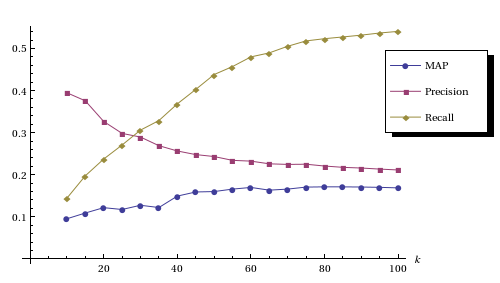
\includegraphics[scale=.65]{tfidfstats}
\caption{Search performance statistics for the systems $S_{F_{tfidf,k}}$.}
\label{filter:fig:tfidfstats}
\end{figure}

%\begin{table}
%\centering
%\begin{footnotesize}
%\begin{tabular}{l|r|r|r|r|r|r}
%\toprule
% & \multicolumn{3}{|c|}{\textbf{True positives}} & \multicolumn{3}{c}{\textbf{False positives}}\\
% \hline
%  & \textit{Abstract} & General & Specific & Abstract & General & Specific\\
%\hline
%Who & & 74& 78& &205 &133\\
%\hline
%What &84 &429 & &396 & 1890&\\
%\hline
%Where & & 37&97 & &152 &624\\
%\hline
%When & & &15 & & &21\\
%\bottomrule
%\end{tabular}
%\caption{Classification of positives for $S_{F_{tfidf,80}}$.}
%\label{filter:table:pan-shat-tfidf}
%\end{footnotesize}
%\end{table}

This section outlines the results for the systems $S_{F_{tfidf,k}}$ which consider only the top $k$ tags for each fragment where the ranking is based on the TF-IDF scores of the tags. We vary the value of $k$ from 10 to 100 with increments of 5. Figure \ref{filter:fig:tfidfstats} presents the search performance statistics as the value of $k$ varies. Not surprisingly, as the value of $k$ increases the search precision and the search recall decrease and increase, respectively. Moreover, the MAP score steadily increases until $k$ equals 80, where the maximal value is reached, and then it starts to decrease. As shown in Table \ref{filter:table:map-prec-rec}, the MAP score of $S_{F_{tfidf,80}}$ is $0.171$ which means it significantly outperforms $SE_{user}$, the systems that indexes all user tags. Indeed, the increase in search performance is 31\%. What is more important is that $S_{F_{tfidf,80}}$ slightly outperforms even $SE_{catalog}$, which until now was the best performing one and the system that we are trying to beat. This suggests that TF-IDF score is indeed a good indication of the quality of the tags and can be used to filter out the bad tags.
%Table \ref{filter:table:pan-shat-tfidf} displays the classification of the results returned by $S_{F_{tfidf,80}}$ according to the Panofsky-Shatford model. What becomes 

\subsection{Network Analysis-based filtering}
\begin{figure}
\centering
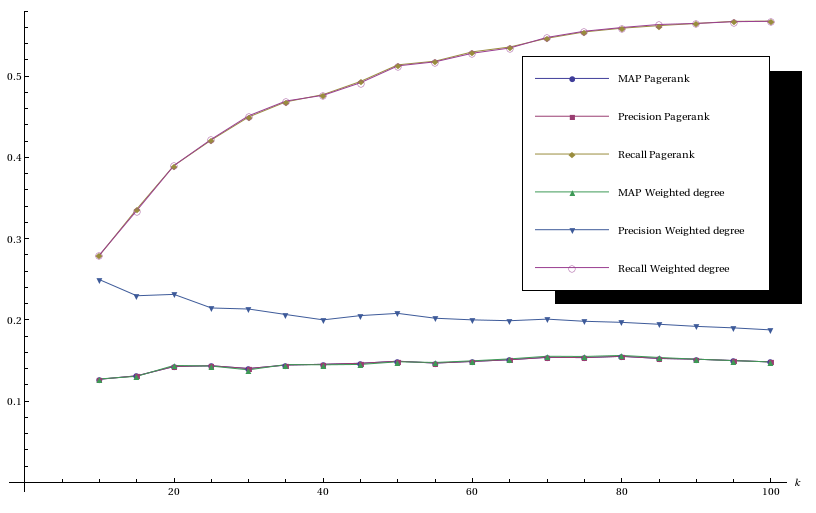
\includegraphics[scale=.45]{filter:netana}
\caption{Search performance statistics for the systems $S_{F_{pagerank,k}}$ and $S_{F_{wdeg,k}}$.}
\label{filter:fig:netana}
\end{figure}
In this section we present the results of the systems $S_{F_{pagerank,k}}$ and $S_{F_{wdeg,k}}$ which consider only the top $k$ tags for each fragment where the ranking is based on the PageRank and weighted degree centrality measures, respectively. The value of $k$ was varied from 10 to 100 with an increment of 5. Figure \ref{filter:fig:netana} summarizes the search performance statistics as the value of $k$ changes. The trends are as expected, as the value of $k$ increase the recall for both systems decreases. On the other hand, the precision drops. The MAP scores for both systems steadily increase and it reaches maximal value at 80. The values of the performance statistics for $S_{F_{pagerank,80}}$ and $S_{F_{wdeg,80}}$ are shown in Table \ref{filter:table:map-prec-rec}. As we can see both systems outperform $SE_{user}$, the system that indexes all user tags. In the case of $S_{F_{pagerank,80}}$ the improvement in terms of the MAP score is 18\% and in the case of $S_{F_{wdeg,80}}$ the improvement in terms of the MAP score is 19\%. This shows that the network centrality is a relatively good indicator of the quality. However while it is a step in the right direction, $SE_{catalog}$ and $S_{F_{tfidf,80}}$ still outperform network-analysis based filtering. Looking at the graphs in Figure \ref{filter:fig:netana} it is striking that the values for the search precision, search recall and MAP for the systems $S_{F_{pagerank,k}}$ and $S_{F_{wdeg,k}}$ as the value of $k$ changes are almost equal. In fact, the difference usually is in the second or the third decimal. This phenomenon can be explained by the structure of the networks that we construct for the fragments. Indeed, the resulting networks usually consists of many isolated well-connected network subcomponents. Consequently, the rankings produced by PageRank and the weighted degree centrality are highly correlated. The structure of the networks is an artefact of DBpedia's classification structure of the articles which is rather sparse: the set of categories is incomplete and not all article-to-category links are present. This prompts us to think that building better networks for semantic connectedness is the key ingredient. Exploiting more of the knowledge encoded in DBpedia or using a different richer knowledge source could perhaps lead to improved detection of the bad tags. 

\subsection{Player reputation-based filtering}
\begin{figure}
\centering
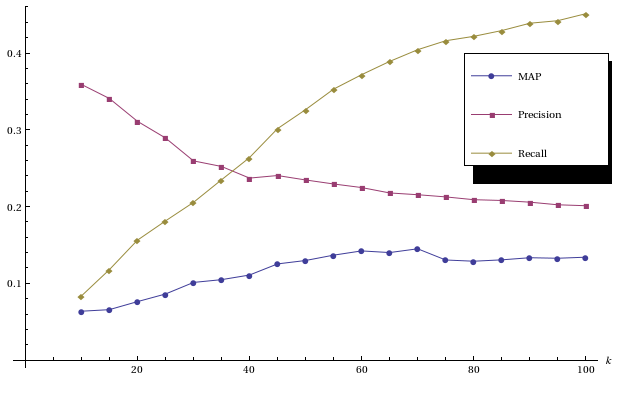
\includegraphics[scale=.5]{filter:rep}
\caption{Search performance statistics for the systems $S_{F_{prep,k}}$.}
\label{filter:fig:reppl}
\end{figure}

\begin{figure}
\centering
\includegraphics[scale=.4]{filter:repcorr}
\caption{Correlation between the reputation and the number of relevant hits for the players. The horizontal axis displays the reputation of the player in increasing order and the vertical axis shows the number of relevant videos retrieved using a tag entered by the corresponding player.}
\label{filter:fig:repcorr}
\end{figure}

This section outlines the results for the system $S_{F_{prep,k}}$ which takes only the top $k$ tags for each fragment where the ranking is based on the combination of the TF-IDF score and the reputation of the players.
As previously, the value of $k$ was varied from 10 to 100 with an increment of 5. Figure \ref{filter:fig:reppl} displays how the MAP score, search precision and search recall change as a function of $k$. The best results are achieved for $k=70$ and are displayed in Table \ref{filter:table:map-prec-rec}. As we can see there is a an improvement of $11\%$ with respect to the MAP score compared to the system $SE_{user}$ which indexes all user tags. However, the search performance of  $S_{F_{prep,70}}$ is worse for all three metrics than the system $S_{F_{tfidf,80}}$ which ranks and filters the tags based only on their TF-IDF scores. This means that considering the reputations of the players in combination with the TF-IDF ranking in this case only worsened the matters for the TF-IDF based filtering. Figure \ref{filter:fig:repcorr} shows the correlation between the reputation of the players and their success in providing tags that resulted in relevant search results. In particular, the horizontal axis shows the reputation for each of the users in increasing order whereas the vertical axis presents the number of relevant video fragments that can be retrieved using tags entered by the corresponding player. As seen, higher reputation does not entail higher success rate. In fact, many of the most  reputable players are among the ones that were the least successful. This means that computing reputation in the manner outlined above may not be the best predictor for the ability of the player to provide topically relevant tags. Alternative explanation is that there is not sufficient data available to reliably estimate the reputation of the players. Recall that 99\% of the players are registered as anonymous and the only data available for them is a single session of playing \textit{Waisda?}.

\section{Conclusions}\label{filter:sec:con}
In this study we have looked into ways we can detect and filter out bad tags and thereby improve the search performance of the video fragment retrieval based on the tags collected by the \textit{Waisda?} video labelling game.

The first direction that we took was to relax the tag verification criterion incorporated in the game. Our previous research had suggested that it is in fact rather limiting and results in omitting good tags. We made two attempts in this direction. The first attempt was to retain the tags that were entered by at least two different players. The second attempt was to keep the tags that were entered at least two times possibly by the same player. Unfortunately, neither proved to be an efficient way of detecting the good tags. The main reason for this is that even though they relax the verification criterion they are still too restricted, thus using all \textit{Waisda?} tags for search is a much better option.

The second direction that we looked into was to exploit background knowledge to filter out the bad tags. In particular, we used the GTAA thesaurus which is employed by the catalogers from the S\&V institute in the process of video annotation. The tag filtering was carried out by keeping only the tags that are present in the GTAA thesaurus. However, this turned out be a bad tag quality predictor as well. The main reason being the low overlap between the \textit{Waisda?} tags and the GTAA thesaurus. In fact, after the filtering for more than half or the queries no results were returned. This result reaffirms the conclusions from Chap. \ref{chap:kcap} about the disparity of the vocabularies used by professionals and normal users and the search gap that spawns from this disparity.

The third direction we investigated was to exploit the standard information retrieval metrics TF-IDF which reflects the importance of a word with respect to a document in a corpus of documents. The filtering is carried out for each video fragment by retaining only the top $k$ tags where the ranking is based on the TF-IDF score of the tags. It turned out that TF-IDF score is a good predictor for the quality of the tags. Indeed, for the case of $k = 80$ we obtained a search performance which is for 31\% better than the search performance of all \textit{Waisda?} tags and marginally better than the search based on the catalog data. If you recall the latter was the best performing when it comes to topical search. This means that the system $S_{F_{tfidf,80}}$ can emulate the search performance of the system $SE_{catalog}$ which is the best performing system when it comes to topical search that does not exploit user tags. 

The fourth direction we undertook was to use the social network analysis tools to characterise the quality of the tags and identify the bad ones. The filtering procedure consisted of the phases. In the first phase we constructed a network that represents the semantic connectedness of the tags in the video using DBpedia as background knowledge. Afterwards, in the second phase we ranked the tags based on their network centrality measure scores and retained only the top $k$ ones. This method of filtering proved to be an improvement over using all \textit{Waisda?} tags. However, it still performed worse than the retrieval based on the catalog data. We hypothesize that this is a consequence of the manner we build the network of semantic connectedness. Constructing a network that bears a better resemblance to the true semantic connectedness relation could yield better tag quality detection.

The last direction we examined was to exploit the reputation of the players to find the good tags. The reputation of a player was based on the positive evidence collected for that player. The positive evidence came in the form of the number of verified tags entered by that player. The reputation of the players was combined with the TF-IDF score of a given tag to compute the overall score for that tag. Unfortunately, this combined strategy yielded worse performance than TF-IDF scoring and filtering alone. This suggests that either the reputation computation mechanism we employed is not appropriate or the lack of evidence we had for the players proved to be too detrimental. In fact, the latter would be an obstacle regardless of the reputation mechanism. This could be attributed as a drawback of the design of the game which incorporated players reputation management only to a limited extend.